% For more detailed article preparation guidelines, please see:
% http://f1000research.com/author-guidelines

\documentclass[10pt,a4paper]{article}
\usepackage{f1000_styles}
\usepackage{gensymb}

%% Default: numerical citations
\usepackage[numbers]{natbib}

%% Uncomment this lines for superscript citations instead
% \usepackage[super]{natbib}

%% Uncomment these lines for author-year citations instead
% \usepackage[round]{natbib}
% \let\cite\citep

\usepackage{rotating}
\usepackage{nicefrac}
\usepackage{url}
\def\UrlBreaks{\do\/\do-}

% Can turn off hyperref if it unwanted, but it is generally useful IMO
\usepackage{xr-hyper}
\usepackage{hyperref}
\usepackage{xcolor}
\hypersetup{
    colorlinks,
    linkcolor={red!50!black},
    citecolor={blue!50!black},
    urlcolor={blue!80!black}
}

%\usepackage{xr} % external references (uncomment if not using xr-hyper)
\externaldocument[main]{main}

\begin{document}

\title{Supplemental Material for:\\
Evaluation of predicted Medfly (\textit{Ceratitis capitata}) quarantine length in the United States utilizing degree-day and agent-based models}

\author[1,2]{Travis C. Collier}
\author[1,3]{Nicholas C. Manoukis}
\affil[1]{Daniel K. Inouye US Pacific Basin Agricultural Research
Center (PBARC), United States Department of Agriculture,
Agricultural Research Service,
Hilo, Hawaii, 96720, USA}
\affil[2]{corresponding author; email: Travis.Collier@ARS.USDA.gov}
\affil[3]{email: Nicholas.Manoukis@ARS.USDA.gov}
% Please list all authors that played a significant role in the research involved in the article. Please provide full affiliation information (including full institutional address, ZIP code and e-mail address) for all authors, and identify who is/are the corresponding author(s).

\maketitle
\thispagestyle{fancy}

%\begin{abstract}
%\end{abstract}

%\section*{Keywords}

\tableofcontents

\clearpage

%%%%%%%%%%%%%%%%%%%%%%%%%%%%%%%%%%%%%%%%%%%%%%%%%%%%%%%%%%%%%%%%%%%%%%%%%%%

\section{``Supernorm'' figures}

\subsection{Daily normal of hourly temperatures}
\begin{figure*}[hb!]
\centering
%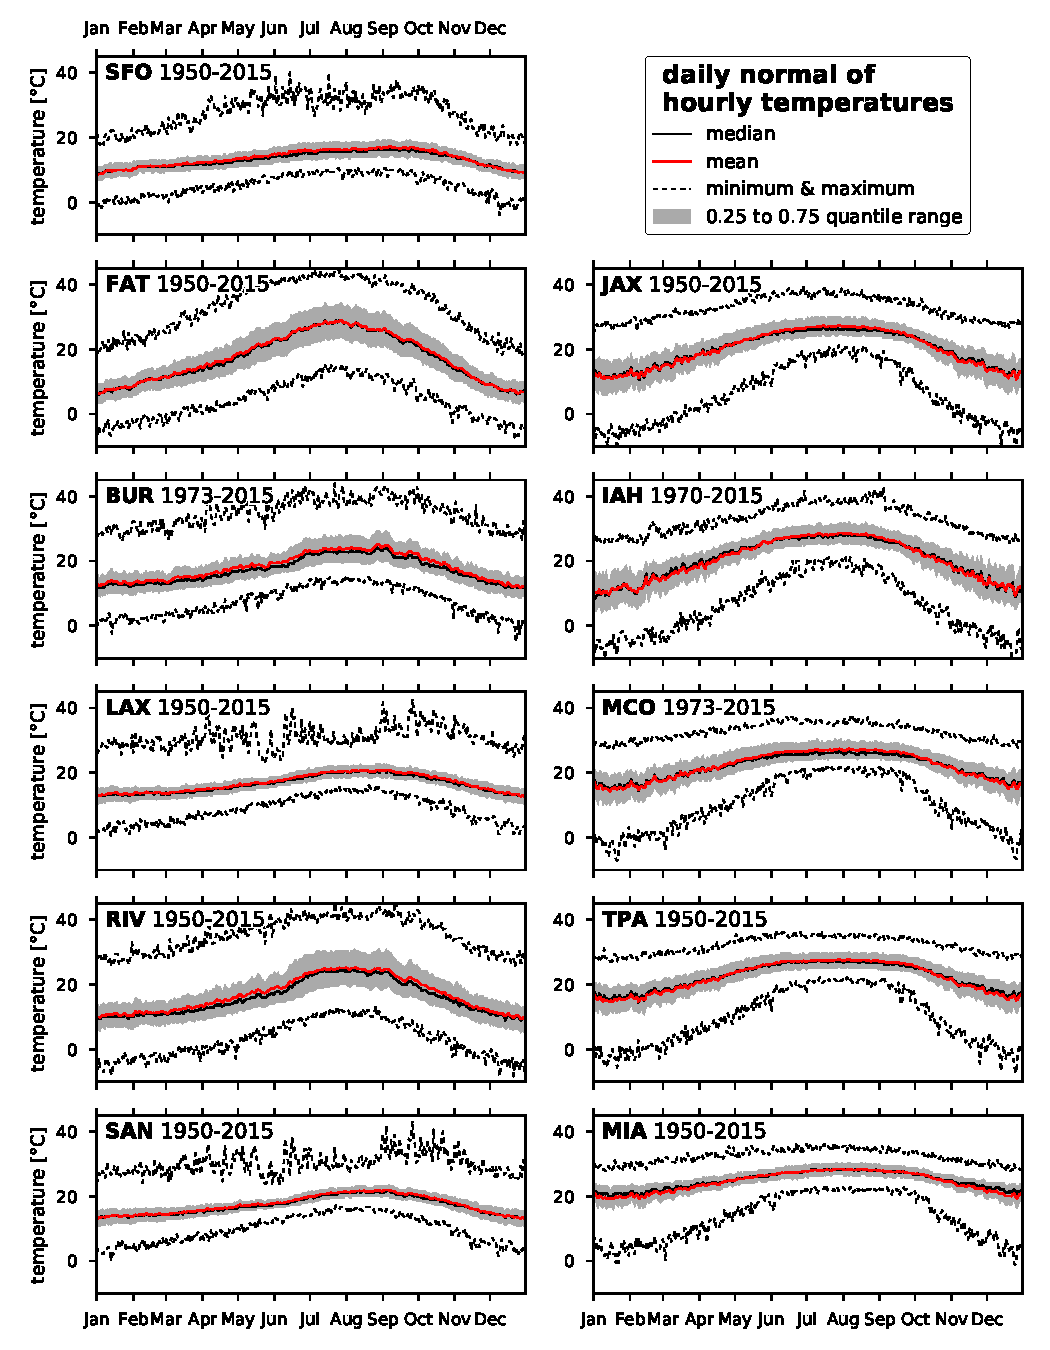
\includegraphics[width=1.0\textwidth]{figs/fig_all_hourly_temps_supernorm.pdf}
% size the figures properly upon generation instead of giving width here, so fonts are proper too @TCC
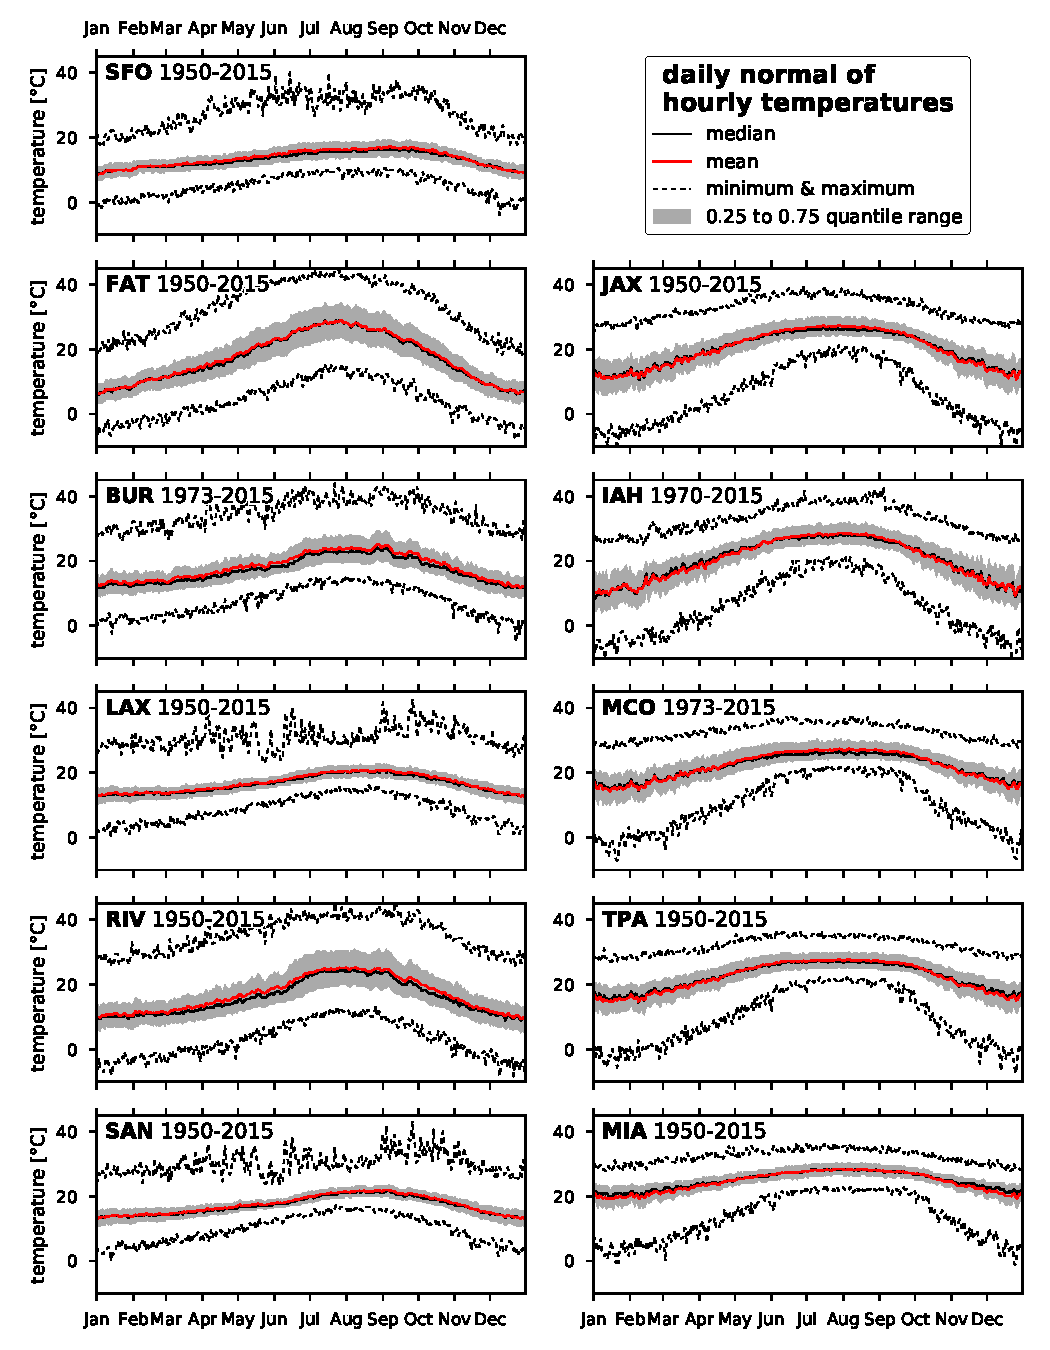
\includegraphics{figs/fig_all_hourly_temps_supernorm.pdf}
\caption{\label{fig:temperature_supernorm}
Hourly temperature data aggregated by day of year.
}
\end{figure*}
\clearpage

\subsection{Degree day based PQL supernorm}
\begin{figure*}[hb!]
\centering
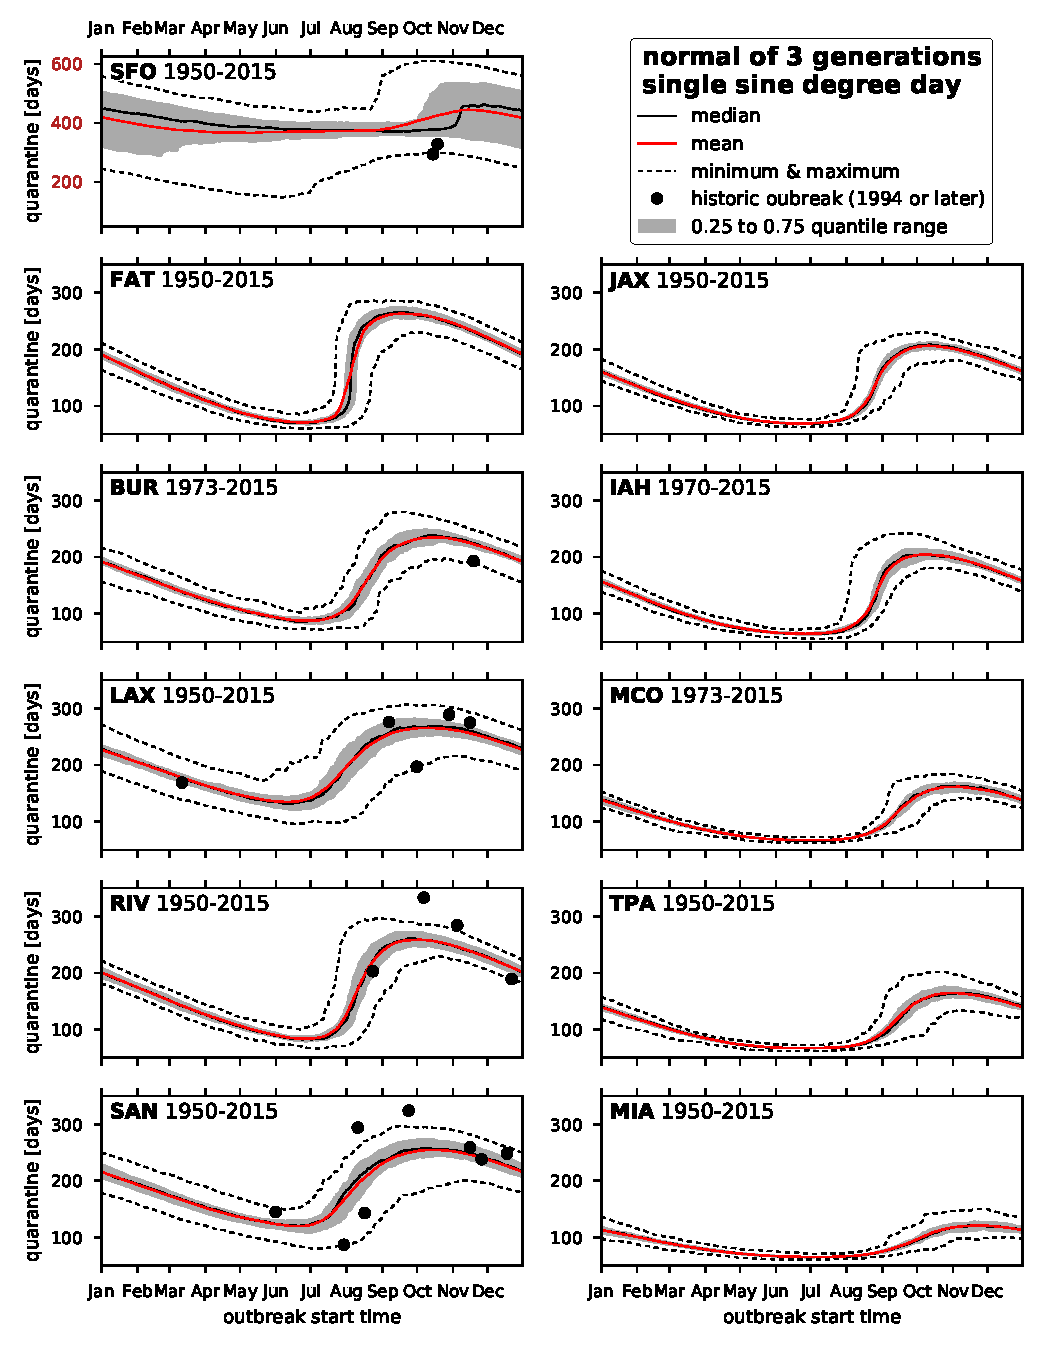
\includegraphics{figs/fig_all_BMDD_supernorm.pdf}
\caption{\label{fig:ddPQL_supernorm}
Single sine degree day based predicted quarantine lengths aggregated by day of year.
}
\end{figure*}
\clearpage

\subsection{MED-FOES PQL based supernorm}
\begin{figure*}[hb!]
\centering
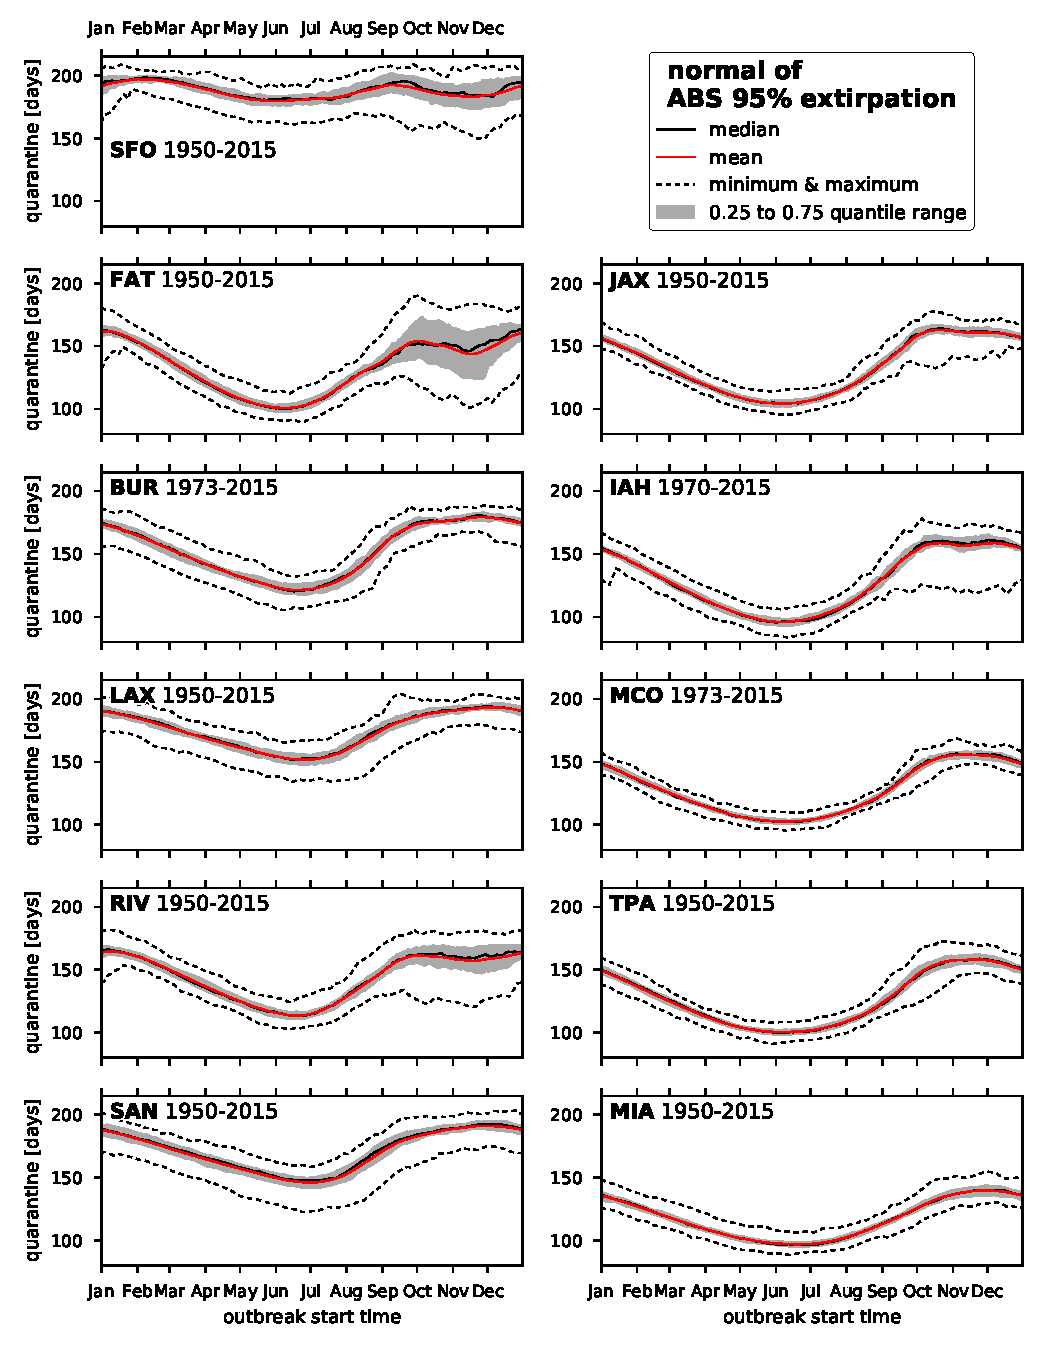
\includegraphics{figs/fig_all_pe95_supernorm.pdf}
\caption{\label{fig:medfoesPQL_supernorm}
MED-FOES based predicted quarantine lengths aggregated by day of year.
}
\end{figure*}
\clearpage


\section{Difference in PQL at nearby sites (LA basin example)}

\begin{figure*}[hb!]
\centering
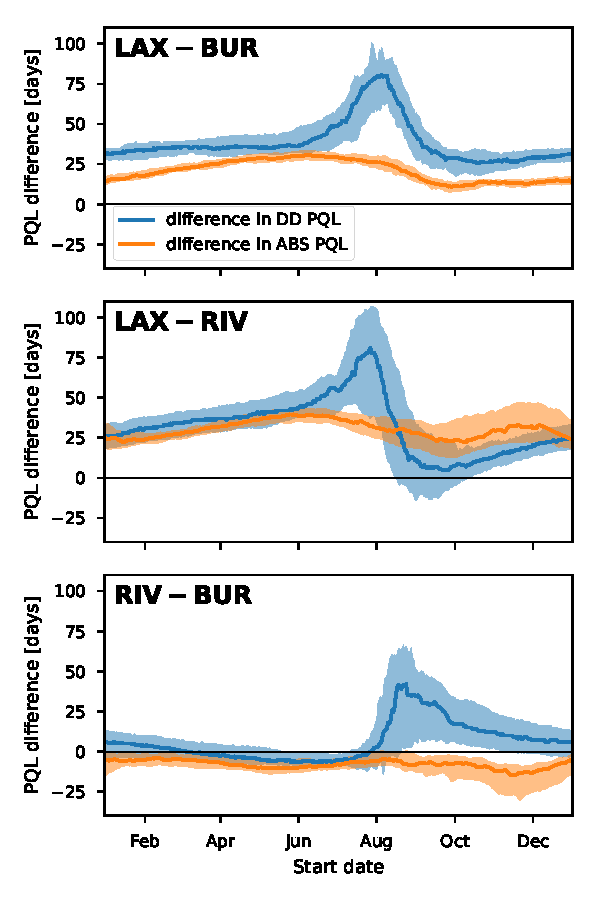
\includegraphics{figs/fig_between_site_differences_LA.pdf}
\caption{\label{fig:PQL_difference_between_sites_LA}
The difference in PQL values for the same start date (including year) between sites in the LA basin. 
For each date over the range of available data
(1973 through 2015 for LAX-BUR and RIV-BUR, 1950 through 2015 for LAX-RIV), PQL values 
for each site are computed and the differences taken.
The resulting differences are then aggregated by day-of-year.
Lines show the median while the shaded region is the 25\% to 75\% quantile
range for each day-of-year aggregation of differences.
}
\end{figure*}
\clearpage



\section{Historical quarantines}
%\begin{sidewaystable}[hb!]
\begin{table}[htb!]
%\hrule \vspace{0.1cm}
\caption{\label{tab:historical_quarantines}Historical quarantines in California.
}
\centering
\rotatebox{90}{
\footnotesize
\begin{tabledata}{llllllrrlrrrr}
\header Year & City & County & Site & Start Date & End Date & Area                    & duration &        day-of-year & DD PQL & mean normal & ABS PQL & mean normal \\
\header      &      &        &      &            &          & [mi\textsuperscript{2}] & [days]   &                    & [days]& DD PQL      & [days]       & ABS PQL \\
\row 1975-1976 &            Venice &     Los Angeles &         KLAX & 1975-11-14 & 1976-08-02 &         100 &   262 & 2011-11-14 &    248 &  257 &  192 &  192 \\
\row      1980 &        Northridge &     Los Angeles &         KBUR & 1980-07-15 & 1980-12-18 &         100 &   156 & 2011-07-15 &     84 &   91 &  123 &  125 \\
\row 1980-1982 &       Santa Clara &     Santa Clara &         KSFO & 1980-07-15 & 1982-09-21 &        3971 &   798 & 2011-07-15 &    365 &  372 &  190 &  182 \\
\row 1987-1988 &   East LA/Maywood &     Los Angeles &         KLAX & 1987-08-21 & 1988-02-05 &         110 &   168 & 2011-08-21 &    218 &  235 &  172 &  170 \\
\row      1988 &        Northridge &     Los Angeles &         KBUR & 1988-07-27 & 1988-11-15 &          62 &   111 & 2011-07-27 &    113 &  102 &  139 &  130 \\
\row 1988-1989 &  West Los Angeles &     Los Angeles &         KLAX & 1988-10-07 & 1989-06-12 &          76 &   248 & 2011-10-07 &    266 &  266 &  191 &  188 \\
\row 1989-1990 &       Elysia Park &     Los Angeles &         KBUR & 1989-08-10 & 1990-11-09 &        1362 &   456 & 2011-08-10 &    117 &  133 &  138 &  138 \\
\row 1989-1990 &     Mountain View &     Santa Clara &         KSFO & 1989-09-11 & 1990-09-14 &          60 &   368 & 2011-09-11 &    359 &  385 &  190 &  192 \\
\row 1991-1996 &       Los Angeles &     Los Angeles &         KLAX & 1991-10-16 & 1996-06-15 &        1576 &  1704 & 2011-10-16 &    231 &  265 &  184 &  189 \\
\row 1992-1993 &          San Jose &     Santa Clara &         KSFO & 1992-08-04 & 1993-10-14 &          62 &   436 & 2011-08-04 &    326 &  373 &  179 &  185 \\
\row      1992 &         Oceanside &       San Diego &         KSAN & 1992-07-04 & 1992-12-15 &          30 &   164 & 2011-07-04 &    103 &  124 &  139 &  146 \\
\row 1994-1995 &         Camarillo &         Ventura &         KBUR & 1994-10-06 & 1995-08-15 &          86 &   313 & 2011-10-06 &    261 &  234 &  177 &  175 \\
\row 1997-1998 &       Walnut Park &     Los Angeles &         KLAX & 1997-10-01 & 1998-04-16 &          69 &   197 & 2011-10-01 &    279 &  265 &  184 &  186 \\
\row 1998-1999 &       Lake Forest &          Orange &         KLAX & 1998-08-06 & 1999-08-27 &          63 &   386 & 2011-08-06 &    227 &  208 &  161 &  162 \\
\row 1998-1999 &           LaJolla &       San Diego &         KSAN & 1998-08-11 & 1999-06-01 &          30 &   294 & 2011-08-11 &    231 &  195 &  165 &  158 \\
\row 1998-1999 &     Lake Elsinore &       Riverside &         KRIV & 1998-11-05 & 1999-08-16 &         180 &   284 & 2011-11-05 &    252 &  246 &  153 &  158 \\
\row 2001-2002 &         Hyde Park &     Los Angeles &         KLAX & 2001-09-07 & 2002-06-10 &          53 &   276 & 2011-09-07 &    285 &  255 &  188 &  179 \\
\row 2005-2006 &  Rancho Cucamonga &  San Bernardino &         KRIV & 2005-10-07 & 2006-09-05 &         204 &   333 & 2011-10-07 &    249 &  258 &  163 &  161 \\
\row 2005-2006 &          San Jose &     Santa Clara &         KSFO & 2005-10-19 & 2006-09-12 &          77 &   328 & 2011-10-19 &    370 &  425 &  201 &  185 \\
\row 2007-2008 &             Dixon &          Solano &         KFAT & 2007-09-17 & 2008-08-08 &         114 &   326 & 2011-09-17 &    267 &  263 &  165 &  148 \\
\row 2007-2008 &          San Jose &     Santa Clara &         KSFO & 2007-10-15 & 2008-08-04 &          75 &   294 & 2011-10-15 &    376 &  422 &  184 &  186 \\
\row 2007-2008 &     Rolling Hills &     Los Angeles &         KLAX & 2007-10-29 & 2008-08-13 &          97 &   289 & 2011-10-29 &    258 &  263 &  190 &  190 \\
\row 2008-2009 &          El Cajon &       San Diego &         KSAN & 2008-11-26 & 2009-07-22 &         107 &   238 & 2011-11-26 &    239 &  240 &  189 &  191 \\
\row 2008-2009 &     Spring Valley &       San Diego &         KSAN & 2008-12-18 & 2009-08-23 &          93 &   248 & 2011-12-18 &    224 &  226 &  187 &  190 \\
\row      2009 &         Mira Mesa &       San Diego &         KSAN & 2009-06-01 & 2009-10-24 &         106 &   145 & 2011-06-01 &    119 &  123 &  148 &  150 \\
\row 2009-2010 &    Imperial Beach &       San Diego &         KSAN & 2009-08-17 & 2010-01-07 &          37 &   143 & 2011-08-17 &    218 &  206 &  161 &  162 \\
\row 2009-2010 &         Escondido &       San Diego &         KSAN & 2009-09-24 & 2010-08-14 &         198 &   324 & 2011-09-24 &    274 &  250 &  185 &  181 \\
\row 2009-2010 &         Fallbrook &       San Diego &         KSAN & 2009-11-16 & 2010-08-02 &          79 &   259 & 2011-11-16 &    273 &  246 &  194 &  191 \\
\row 2009-2010 &      Santa Monica &     Los Angeles &         KLAX & 2009-11-16 & 2010-08-18 &          65 &   275 & 2011-11-16 &    278 &  256 &  193 &  192 \\
\row 2012-2013 &  Rancho Cucamonga &  San Bernardino &         KRIV & 2012-08-24 & 2013-03-15 &          88 &   203 & 2011-08-24 &    203 &  220 &  131 &  143 \\
\row      2014 &       Los Angeles &     Los Angeles &         KLAX & 2014-03-12 & 2014-08-28 &          88 &   169 & 2011-03-12 &    149 &  177 &  163 &  174 \\
\row 2014-2015 &            Perris &       Riverside &         KRIV & 2014-12-22 & 2015-06-29 &          83 &   189 & 2011-12-22 &    193 &  210 &  164 &  162 \\
\row 2015-2016 &           La Mesa &       San Diego &         KSAN & 2015-07-30 & 2015-10-25 &          93 &    87 & 2011-07-30 &     89 &  167 &  129 &  152 \\
\row 2016-2017 &            Arleta &     Los Angeles &         KBUR & 2016-11-19 & 2017-05-31 &         127 &   193 & 2011-11-19 &    220 &  223 &  158 &  179 \\
\end{tabledata}
} % close rotatebox{90}
\end{table}
\end{document}
